\documentclass[UFT8]{ctexart}
\setCJKmainfont[BoldFont=STHeiti,ItalicFont=STKaiti]{STSong}%\fangsong \songti  \heiti \kaishu \wuhao \small \large \LARGE
\usepackage{graphicx} % 导入插图功能
\usepackage{float}
\usepackage{threeparttable}
\usepackage{caption}
\usepackage{subfigure}
\usepackage{amsmath}
\usepackage{diagbox} % \diagbox[斜线方形]{分区1内容}{分区2内容}{分区3内容}...
\usepackage{ulem}
\usepackage{ctex}
\usepackage{booktabs}% \toprule \midrule \bottomrule
\usepackage{multirow}% \multicolumn{}{}{}
\usepackage{ulem}%\xout 斜删除线 \sout 删除线 \uline下划线 \uuline 双下划线 \uwave 波浪线 

\usepackage{color}
\def\red{\textcolor{red}}
\def\blue{\textcolor{blue}}
\definecolor{green}{RGB}{0,153,51}
\def\green{\textcolor{green}}

\def\bi{\begin{itemize}}
\def\ei{\end{itemize}}
\def\be{ \begin{enumerate}}
\def\ee{ \end{enumerate}}

\usepackage{hyperref}
\hypersetup{
    colorlinks=true,
    linkcolor=blue,
    filecolor=blue,
    urlcolor=black,
    pdftitle={Overleaf Example},
%    pdfpagemode=FullScreen,
    }
\urlstyle{same}
\def\link{\hyperlink}
\def\target{\hypertarget}


\headsep 0.5 true cm \topmargin 0pt \oddsidemargin 0pt
\evensidemargin 0pt \textheight 215mm \textwidth 155mm

\begin{document}

\thispagestyle{empty} 
\vspace*{3cm}
\begin{center}
{{\LARGE\heiti 2023年中国人民大学博士申请材料}\\[0.6cm]
{\normalsize 唐洁}\\[0.1cm]
{\small(广西师范大学数学与统计学院, 广西桂林, 541004)}}
\end{center}

\clearpage%新的一页
\tableofcontents%输出目录
\thispagestyle{empty} % 当前页不显示页码


\clearpage%新的一页
\setcounter{page}{1}%设置首页

\clearpage%新的一页
\section{简历}

\bigskip
\begin{center}
{ \bf \kaishu \large  自我介绍}
\end{center}

我,九五后,湖南人,小个子,五口人,血型AB,钝反应,擅坚持,爱自由,能牺牲。

我的成绩排名第一,根据大多数普通高校绩点\href{https://tang-jay.github.io/certificate/GPA.pdf}{\uline{计算方式}},可得本人所修全部学科GPA:4.05,所修专业学科GPA:4.12。

我是一个对他人、对自己有责任感的人。对他人,我会认真听取他人意见,倾听他人烦恼,为他人排忧解难。在得到他人的帮助的快乐中,学会换位思考,学会助人。对自己,我会安排好自己的时间,先做好自己该做的事,再做自己喜欢的事。

我是一个对集体、对家人有使命感的人。对集体,我觉得自己有义务有力出力,为了集体的荣誉不计较个人得失。对家人,我身为家中最大的小孩,一直觉得自己应该做好榜样,以身作则,给家人一个放心的依靠。

我对自己未来的期盼,就是不论日后成就是高是低,学识是深是浅,担子是多是少,自己可以竭尽所能,遇山开路逢水架桥,提高解决问题的能力,做到问心无愧,不辜负于人,不辜负自己。

\bigskip
\begin{center}
{ \bf \kaishu \large   联系方式}
\end{center}

邮箱地址: 1243711126@qq.com     \quad    手机号码:18177330073    \quad  微信号:与手机号相同

\bigskip
\begin{center}
{ \bf \kaishu \large   个人履历}
\end{center}
 
{\center \bf \kaishu     2020-09~至今 \quad 广西师范大学 \quad  统计学(硕士)}
\smallskip

\bi
\item 主修科目:应用随机过程,高等数理统计,高等概率论,极限理论,统计学习方法,统计软件与计算,应用回归分析,应用时间序列分析,现代非参数统计,抽样调查方法与应用,统计学案例研究,金融工具,数理金融,中级计量经济学,多元统计分析课程。
\item 努力方向:除了课内的学习,课外主要的事情就是专一地写论文,附带培养自己编程的爱好。
\bi
\item 在2020.09 至 2022.06期间,已发表 1 篇中文普刊,已有 3 篇论文正在投稿,其中包含一篇中文,两篇英文。目前有一篇论文正在定稿。
\item 在2021.12申请了院级立项项目,计划 2022.12完成项目。 

\item 学习 Python 掌握爬虫、自动化办公等技能,利用所学技能搭建模型(如漏斗分析模型、RFM用户分析模型等)做数据分析。
\item leetcode 刷题(因为大部分精力在写论文,所以刷题并不多)。
\item  出于兴趣购买网课了解部分机器视觉的知识。
\item  掌握 git 基本命令。
 \item 掌握 Hugo 搭建网站,例如我的\href{https://tang-jay.github.io}{\uline{个人网站}}。
\ei
\ei

{\center \bf \kaishu      2017-09~2020-06 \quad  灵官镇大同市中学 \quad  乡村特岗教师(工作)}
\smallskip
 
\bi
\item 工作内容:班主任,数学教师。
\item 工作感悟:这段经历是个慢生活,晨光会洒满你的窗台,余晖会晕染整个天空,暴风雷电会响彻整个屋顶,我在这样一片自然风光里与学生们相处。与其说我是教学生,真的不如说是学生教我。我见他们如见自己。当他们因为数学题头大的时候,我发现自己也曾因畏惧数学而忽略了动手;当学生否定自己的时候,我发现自己也总在不经意间就不自信了;当学生只想玩手机不读书的时候,我发现曾经许多光阴就是这样自以为是地虚度了。我也是由他们成长过来的,我把学生看作曾经那个自己,与他们交流就是想告诉他们,时光倒流的话我会这样做吧——要动手要自信要读点书,同样也是告诉现在的自己要勇敢要坚韧要明事理。
\ei

{\center \bf \kaishu       2013-09~2017-06 \quad   衡阳师范学院  \quad 数学与应用数学(本科)}
\smallskip
  
\bi
\item 主修科目:数学分析,高等代数,抽象代数,数理统计,常微分方程,数学软件与实验,MATLAB与建模,教师心理学,教育学,初等几何研究等课程。
\item 本科感悟:除了课内学习,我还参加了许多课外活动,比如:考证(C++程序语言设计国家计算机二级等级证书、会计从业资格证、英语四级),比赛(数学建模、演讲比赛、英语演讲比赛、辩论赛、数学竞赛),练习口语(参加点亮英语集训营)、创业(一分钟快照)、实习(祁东启航学校中学部)等等。这一时期,我把自己塞得满满当当的,因为不知道自己怎样做是最好,就都尝试一遍。回头看,还是很感谢这段时间的自己,虽然有些盲目但一直在努力。 
\ei

\bigskip
\begin{center}
{ \bf \kaishu \large     计算机水平}
\end{center}

对 R、Python 更熟悉。
\bi
\item 语言:R,Python,\sout{MatLab},Hugo
\item 操作系统:日常使用 macOS
\item 计算机等级:
  \bi
   \item 国家计算机二级程序语言设计类之 C++、Python
   \item 国家计算机三级之网络安全
   \ei
\ei

\bigskip
\begin{center}
{ \bf \kaishu \large    英语水平}
\end{center}

通过六级考试,口语未开发过,听力水平欠缺,阅读基本无碍,写作仍需锻炼。

\bigskip
\begin{center}
{ \bf \kaishu \large      目前成果}
\end{center}

{\center \bf \kaishu     已发表论文}
\smallskip

\be
\item 唐洁.含空间自回归误差的空间自回归模型的经验欧氏似然推断[J].广西民族大学学报(自然科学版),2021,27(04):70-74. 
\ee

{\center \bf \kaishu      待发表论文}
\smallskip

\be
\item 唐洁,秦永松.含空间自相关误差的空间自回归模型的调整经验似然推断.
\item Tang Jie, Qin Yongsong. Empirical likelihood for spatial dynamic panel data models with spatial errors and endogenous initial observations.
\item Tang Jie, Qin Yongsong. Adjusted empirical likelihood for probability density functions under strong mixing samples.
\ee

{\center \bf \kaishu       承担课题}

\be
\item 2021年12月立广西研究生教育创新计划项目(YJSCXP202104),承担课题《空间计量经济模型的调整经验似然》,计划2022年12月结题。
\ee

 {\center \bf \kaishu      网络文章}
 
 \bi
\item \href{https://blog.csdn.net/JTang1995?type=lately}{\uline{CSDN文章}} 
\item 在线文章 
   \bi
   \item \href{https://tang-jay.github.io/RBook}{\uline{《R语言画图》}} 
   \item \href{https://tang-jay.github.io/EssayNotes}{\uline{《论文写作听课笔记》}} 
   \ei
\ei

\clearpage
\section{个人自述}
\subsection{个人自述}
\subsection{Self-introduction}


%\clearpage
%%\section{成绩单}
%%\subsection{本科成绩单}
%%\begin{center}
%%  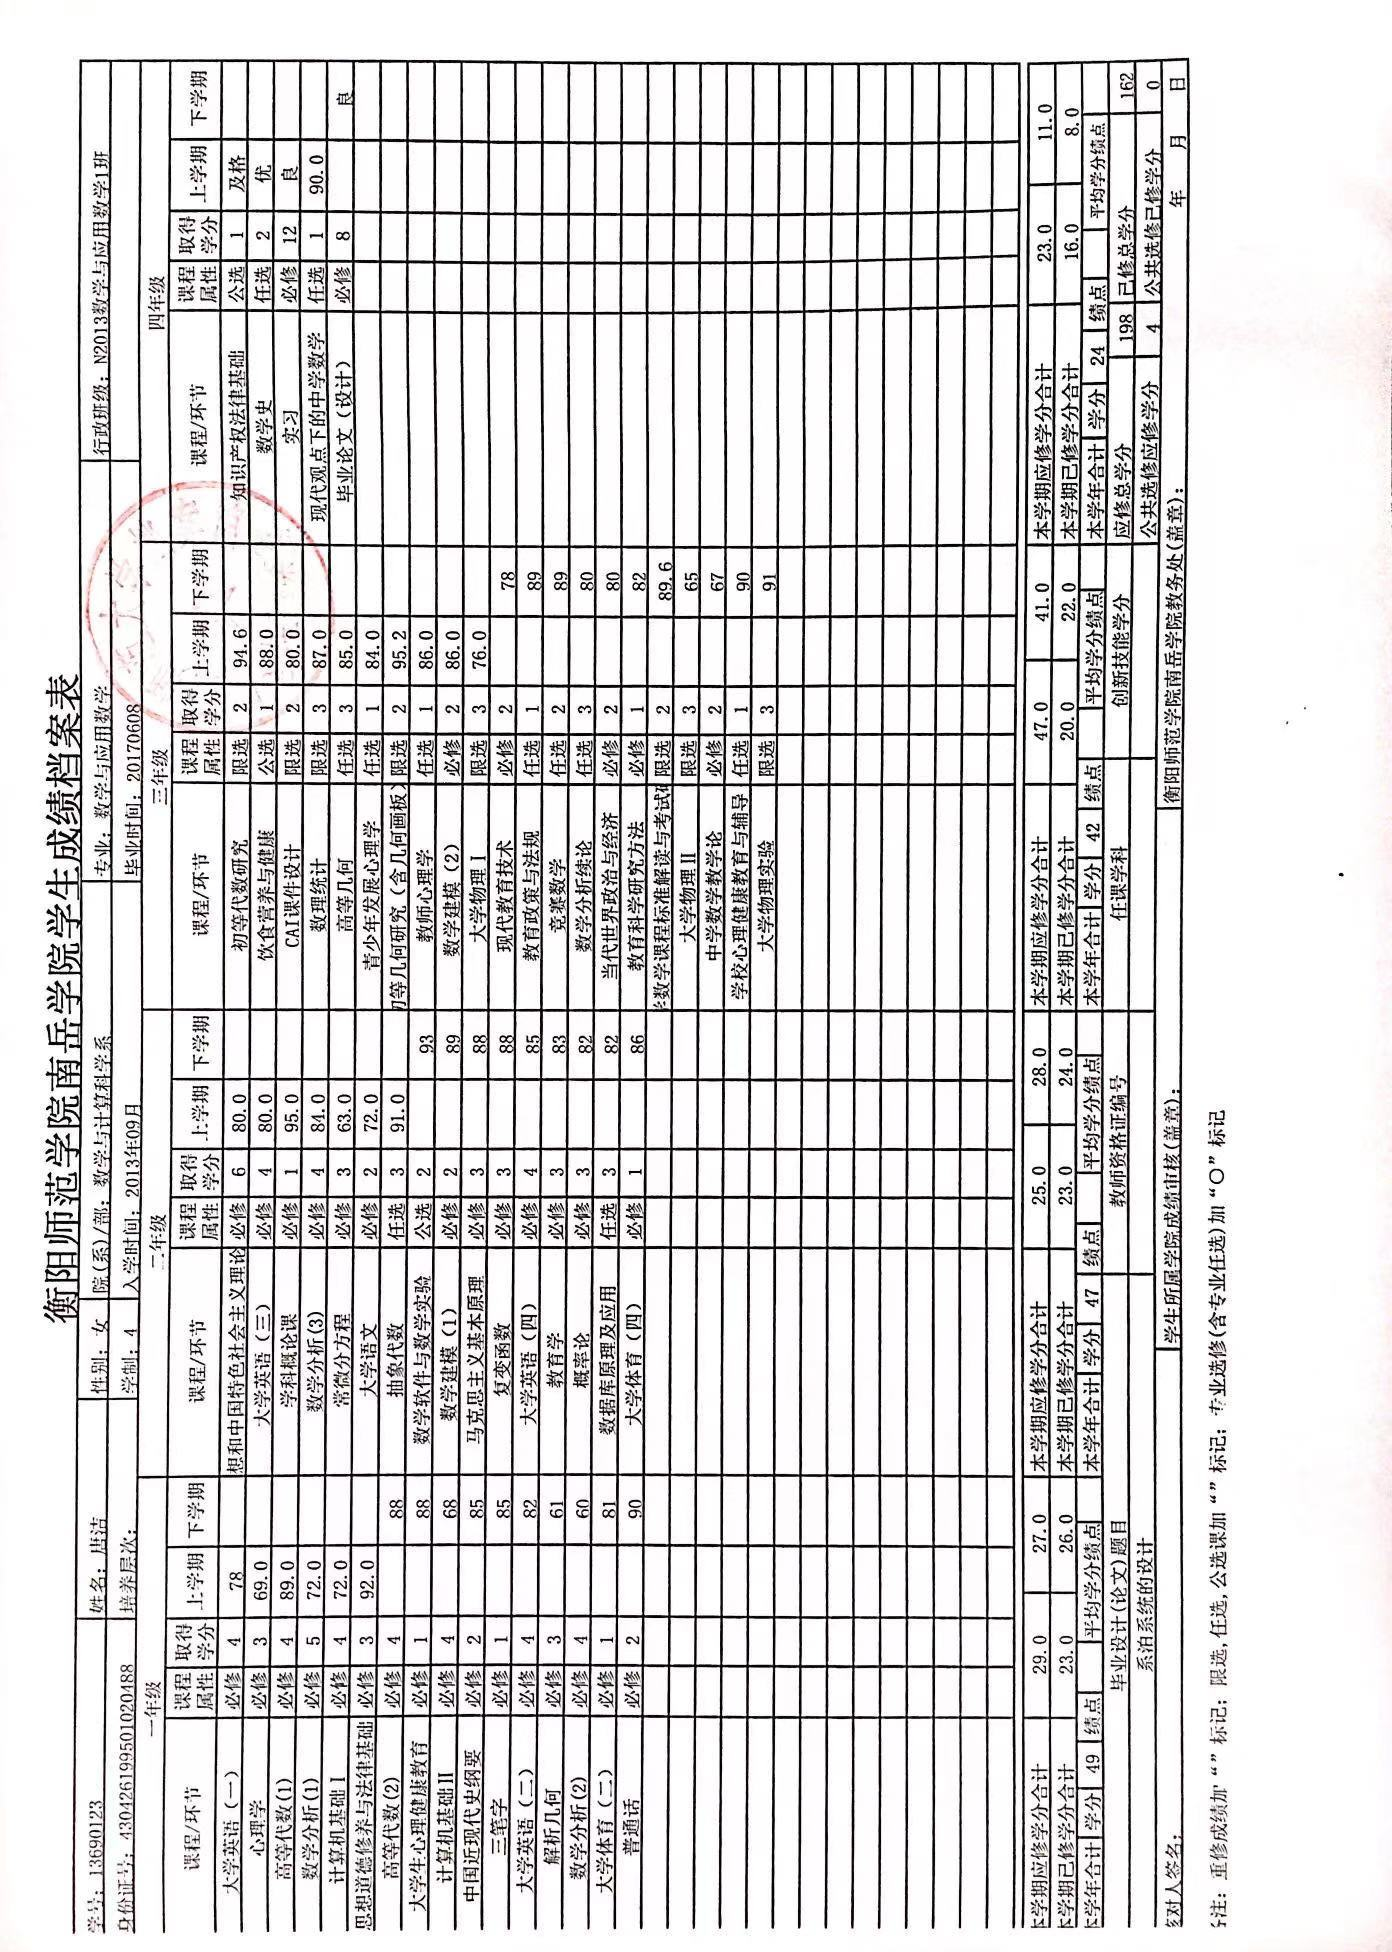
\includegraphics[scale=0.28]{figs/本科成绩单.JPG }
%%\end{center}
%
%\subsection{ 硕士成绩单}
%\begin{center}
%  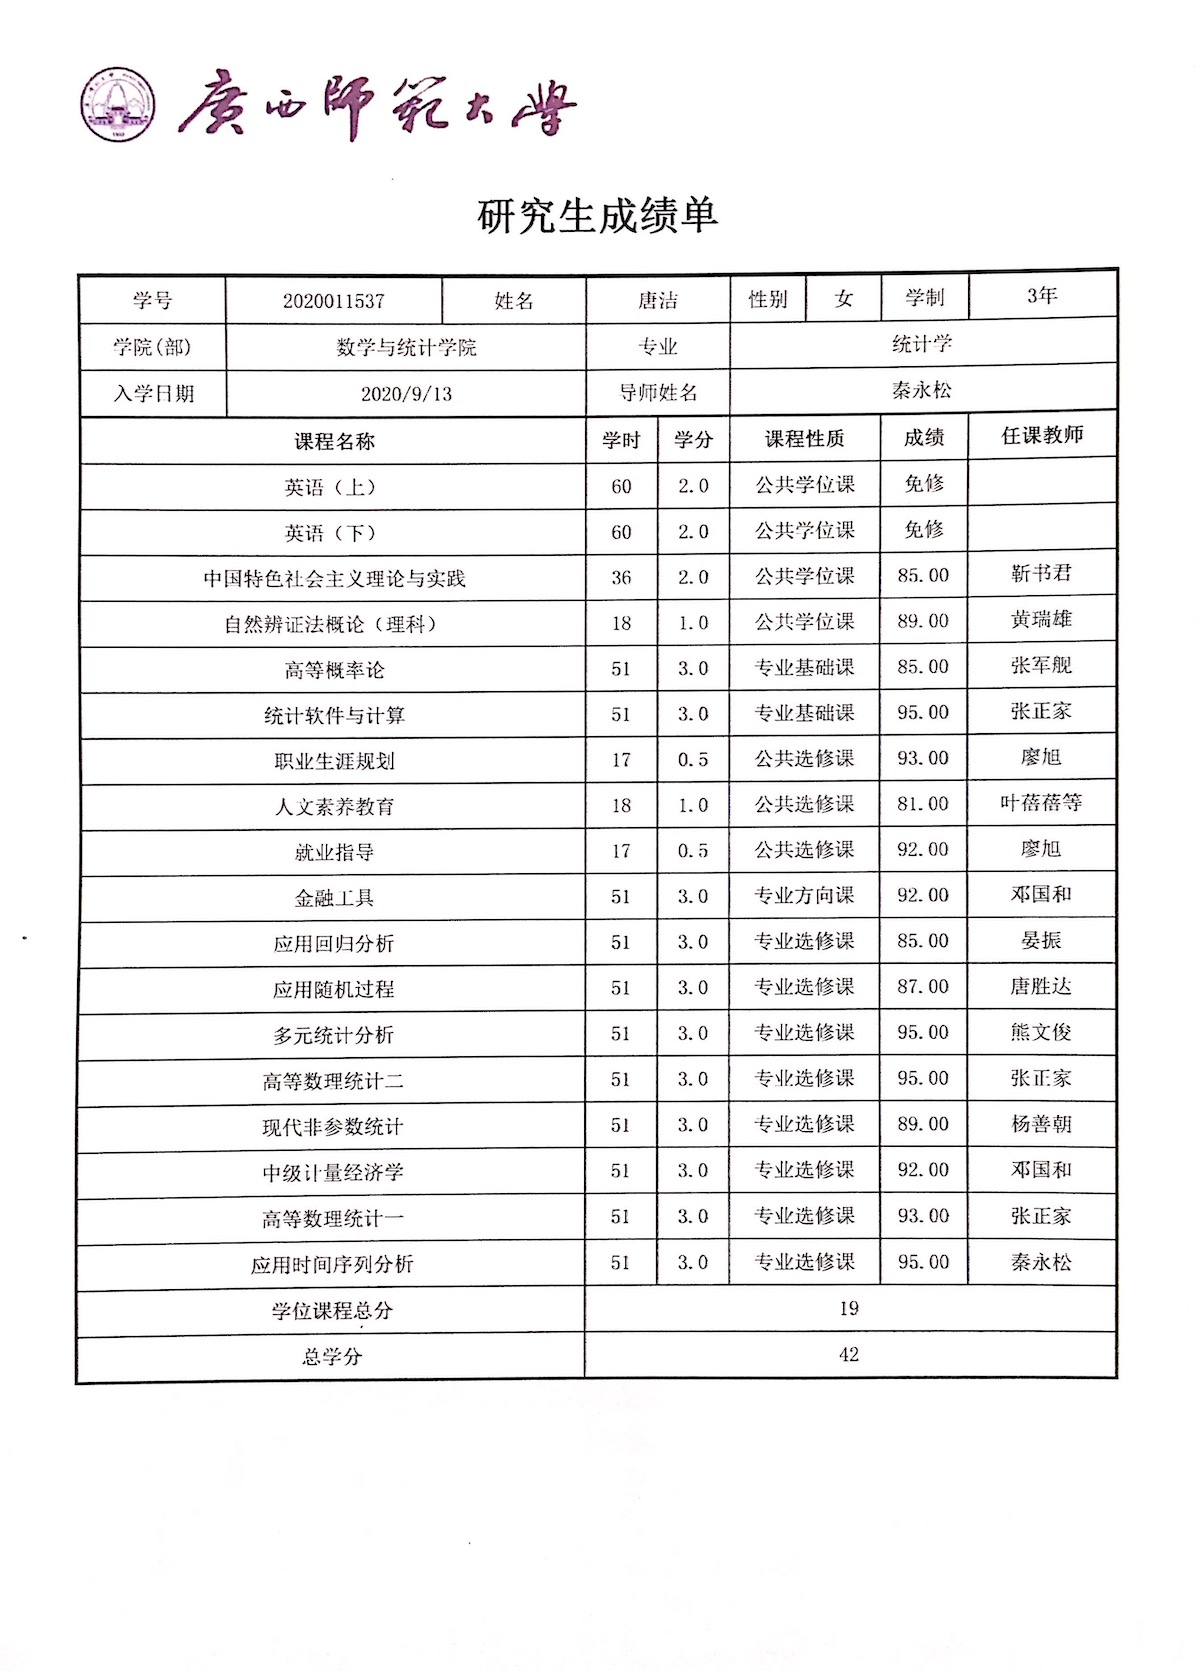
\includegraphics[scale=0.22]{figs/硕士成绩单1.JPG }
%\end{center}
%
%\begin{center}
%  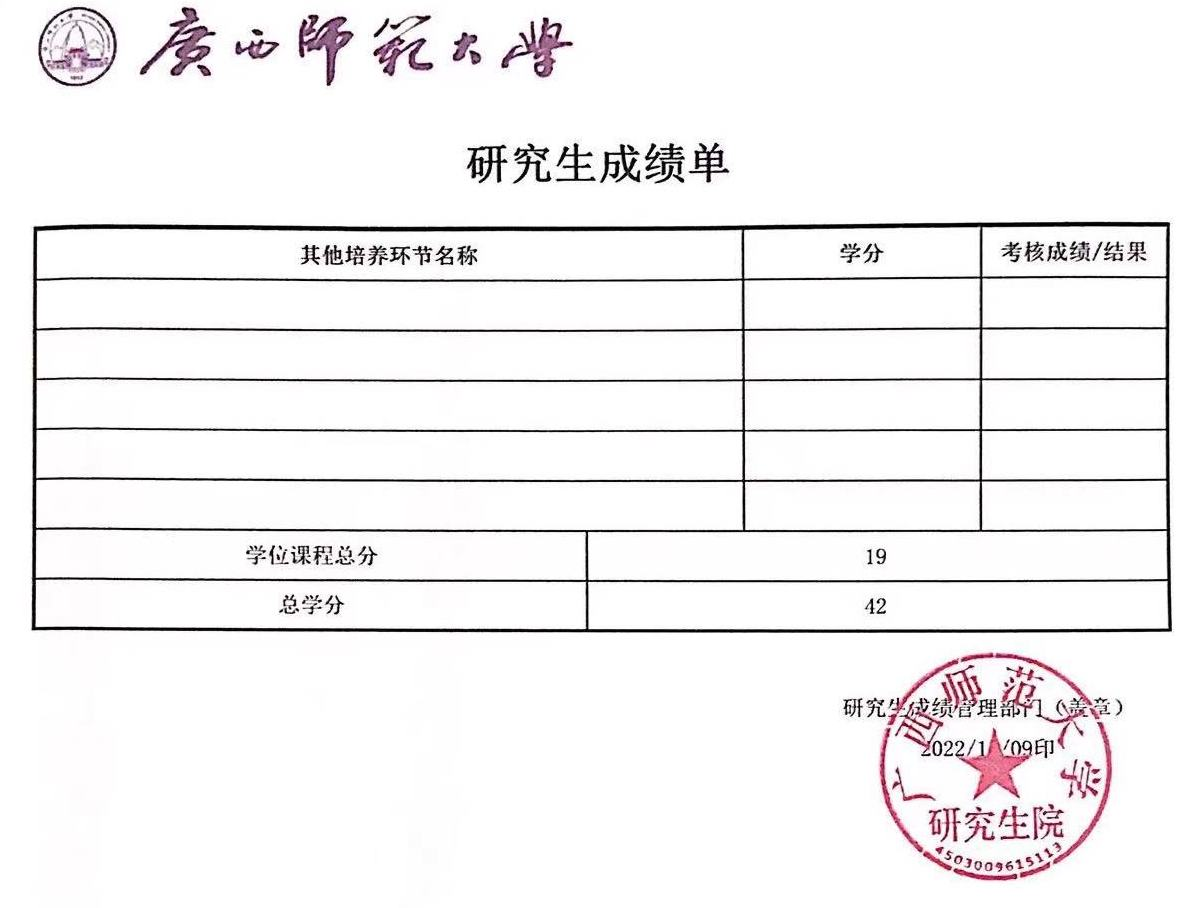
\includegraphics[scale=0.35]{figs/硕士成绩单2.JPG }
%\end{center}



\clearpage
\section{英语六级}
2020年12月通过全国大学英语六级考试

%\begin{center}
%  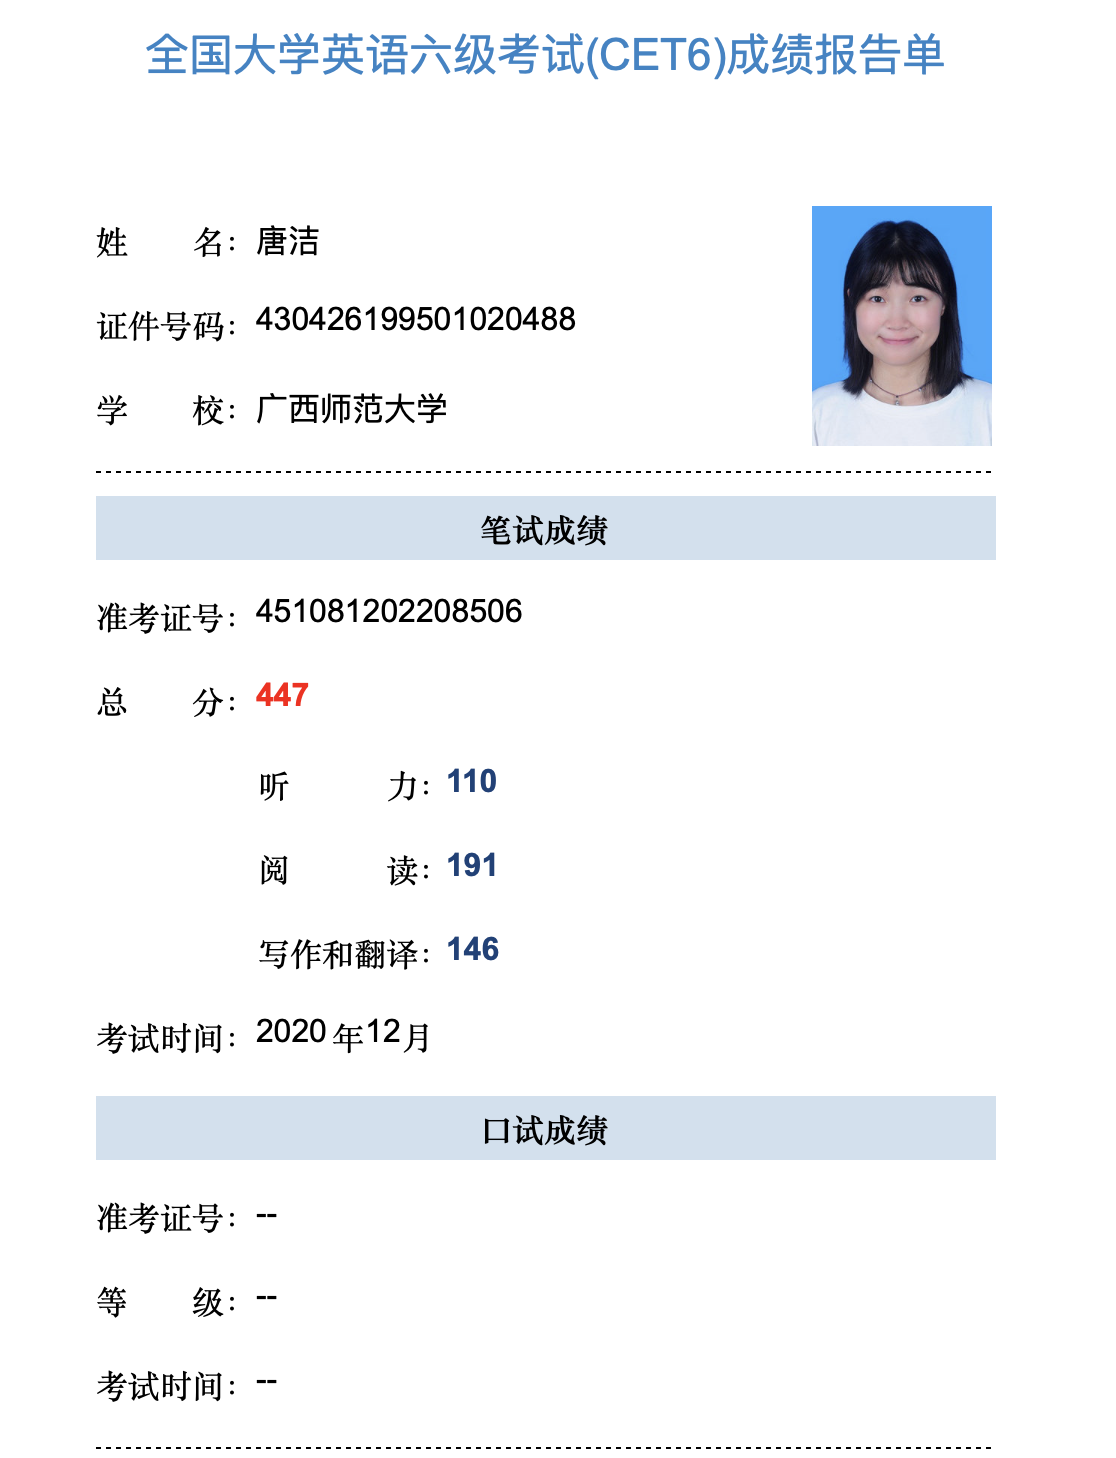
\includegraphics[scale=0.34]{figs/202012.JPG }
%\end{center}

\clearpage
\section{推荐信}
\subsection{第一封}
\clearpage
\subsection{第二封}

\clearpage
\section{硕士学位论文}

\clearpage
\section{应届毕业生材料}
\subsection{本科学历}
%\begin{center}
%  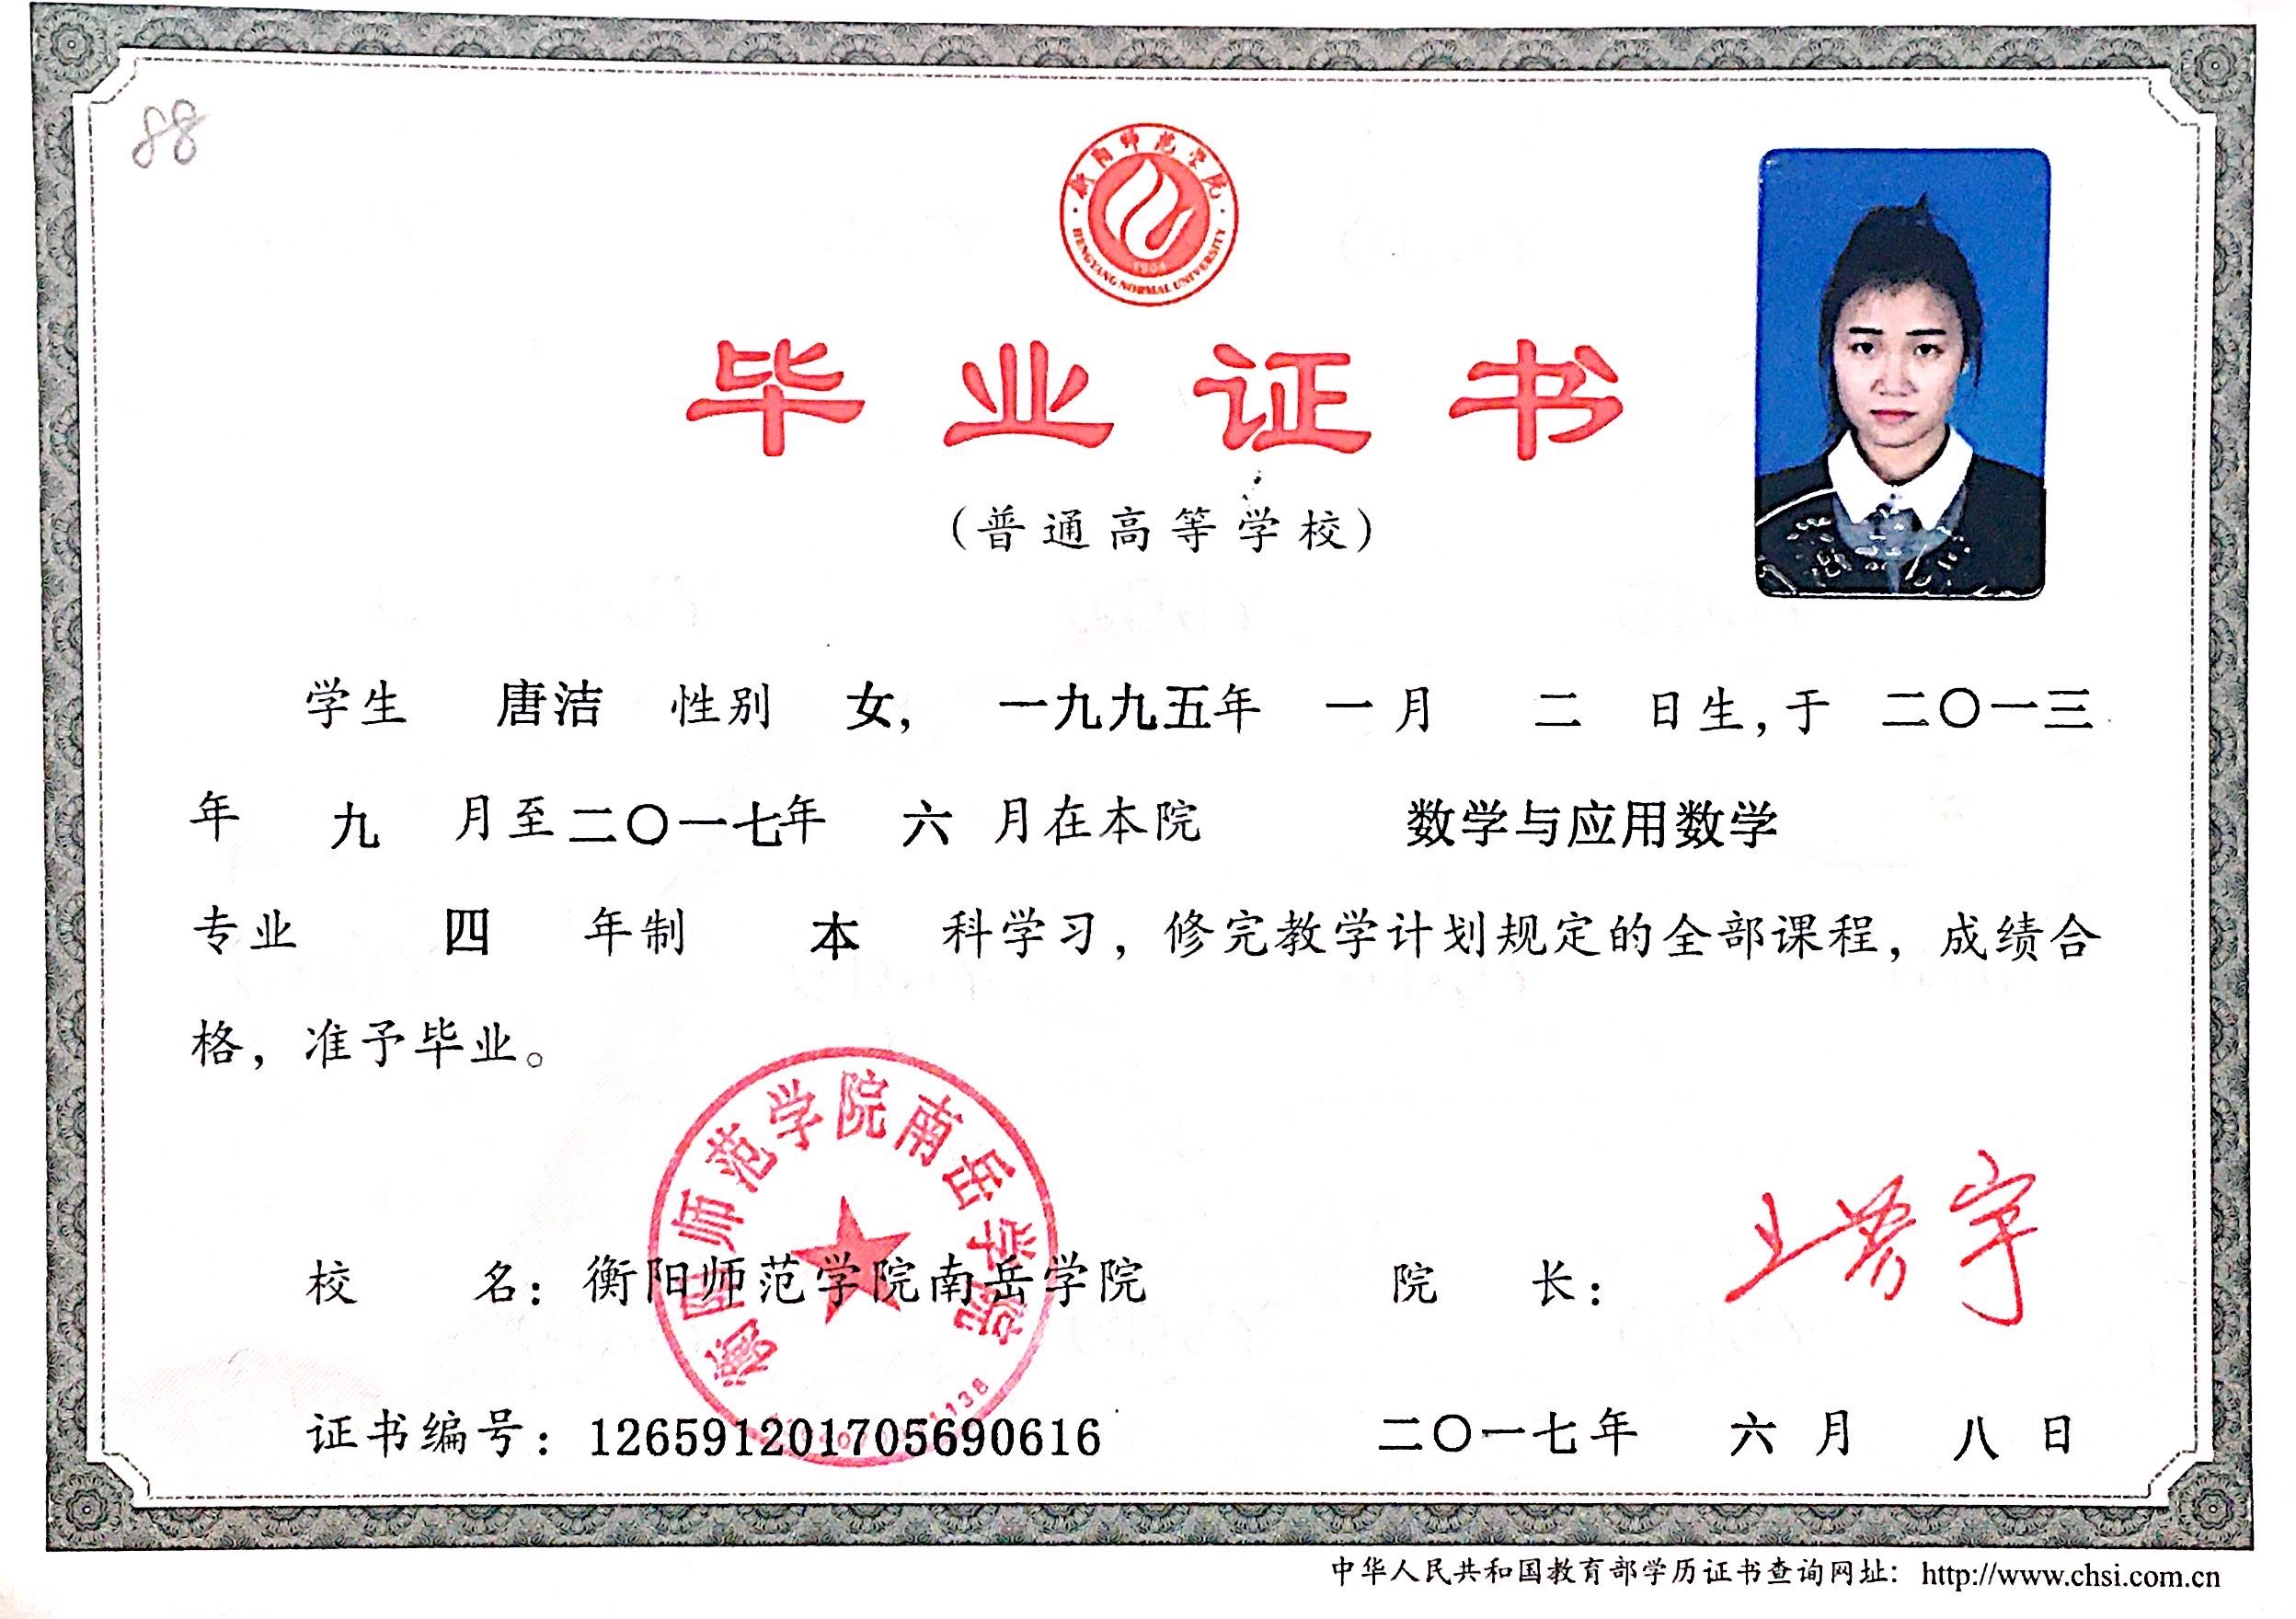
\includegraphics[scale=0.2]{figs/20170608_1.JPG }
%\end{center}

%\subsection{学士学位证书}
%\begin{center}
%  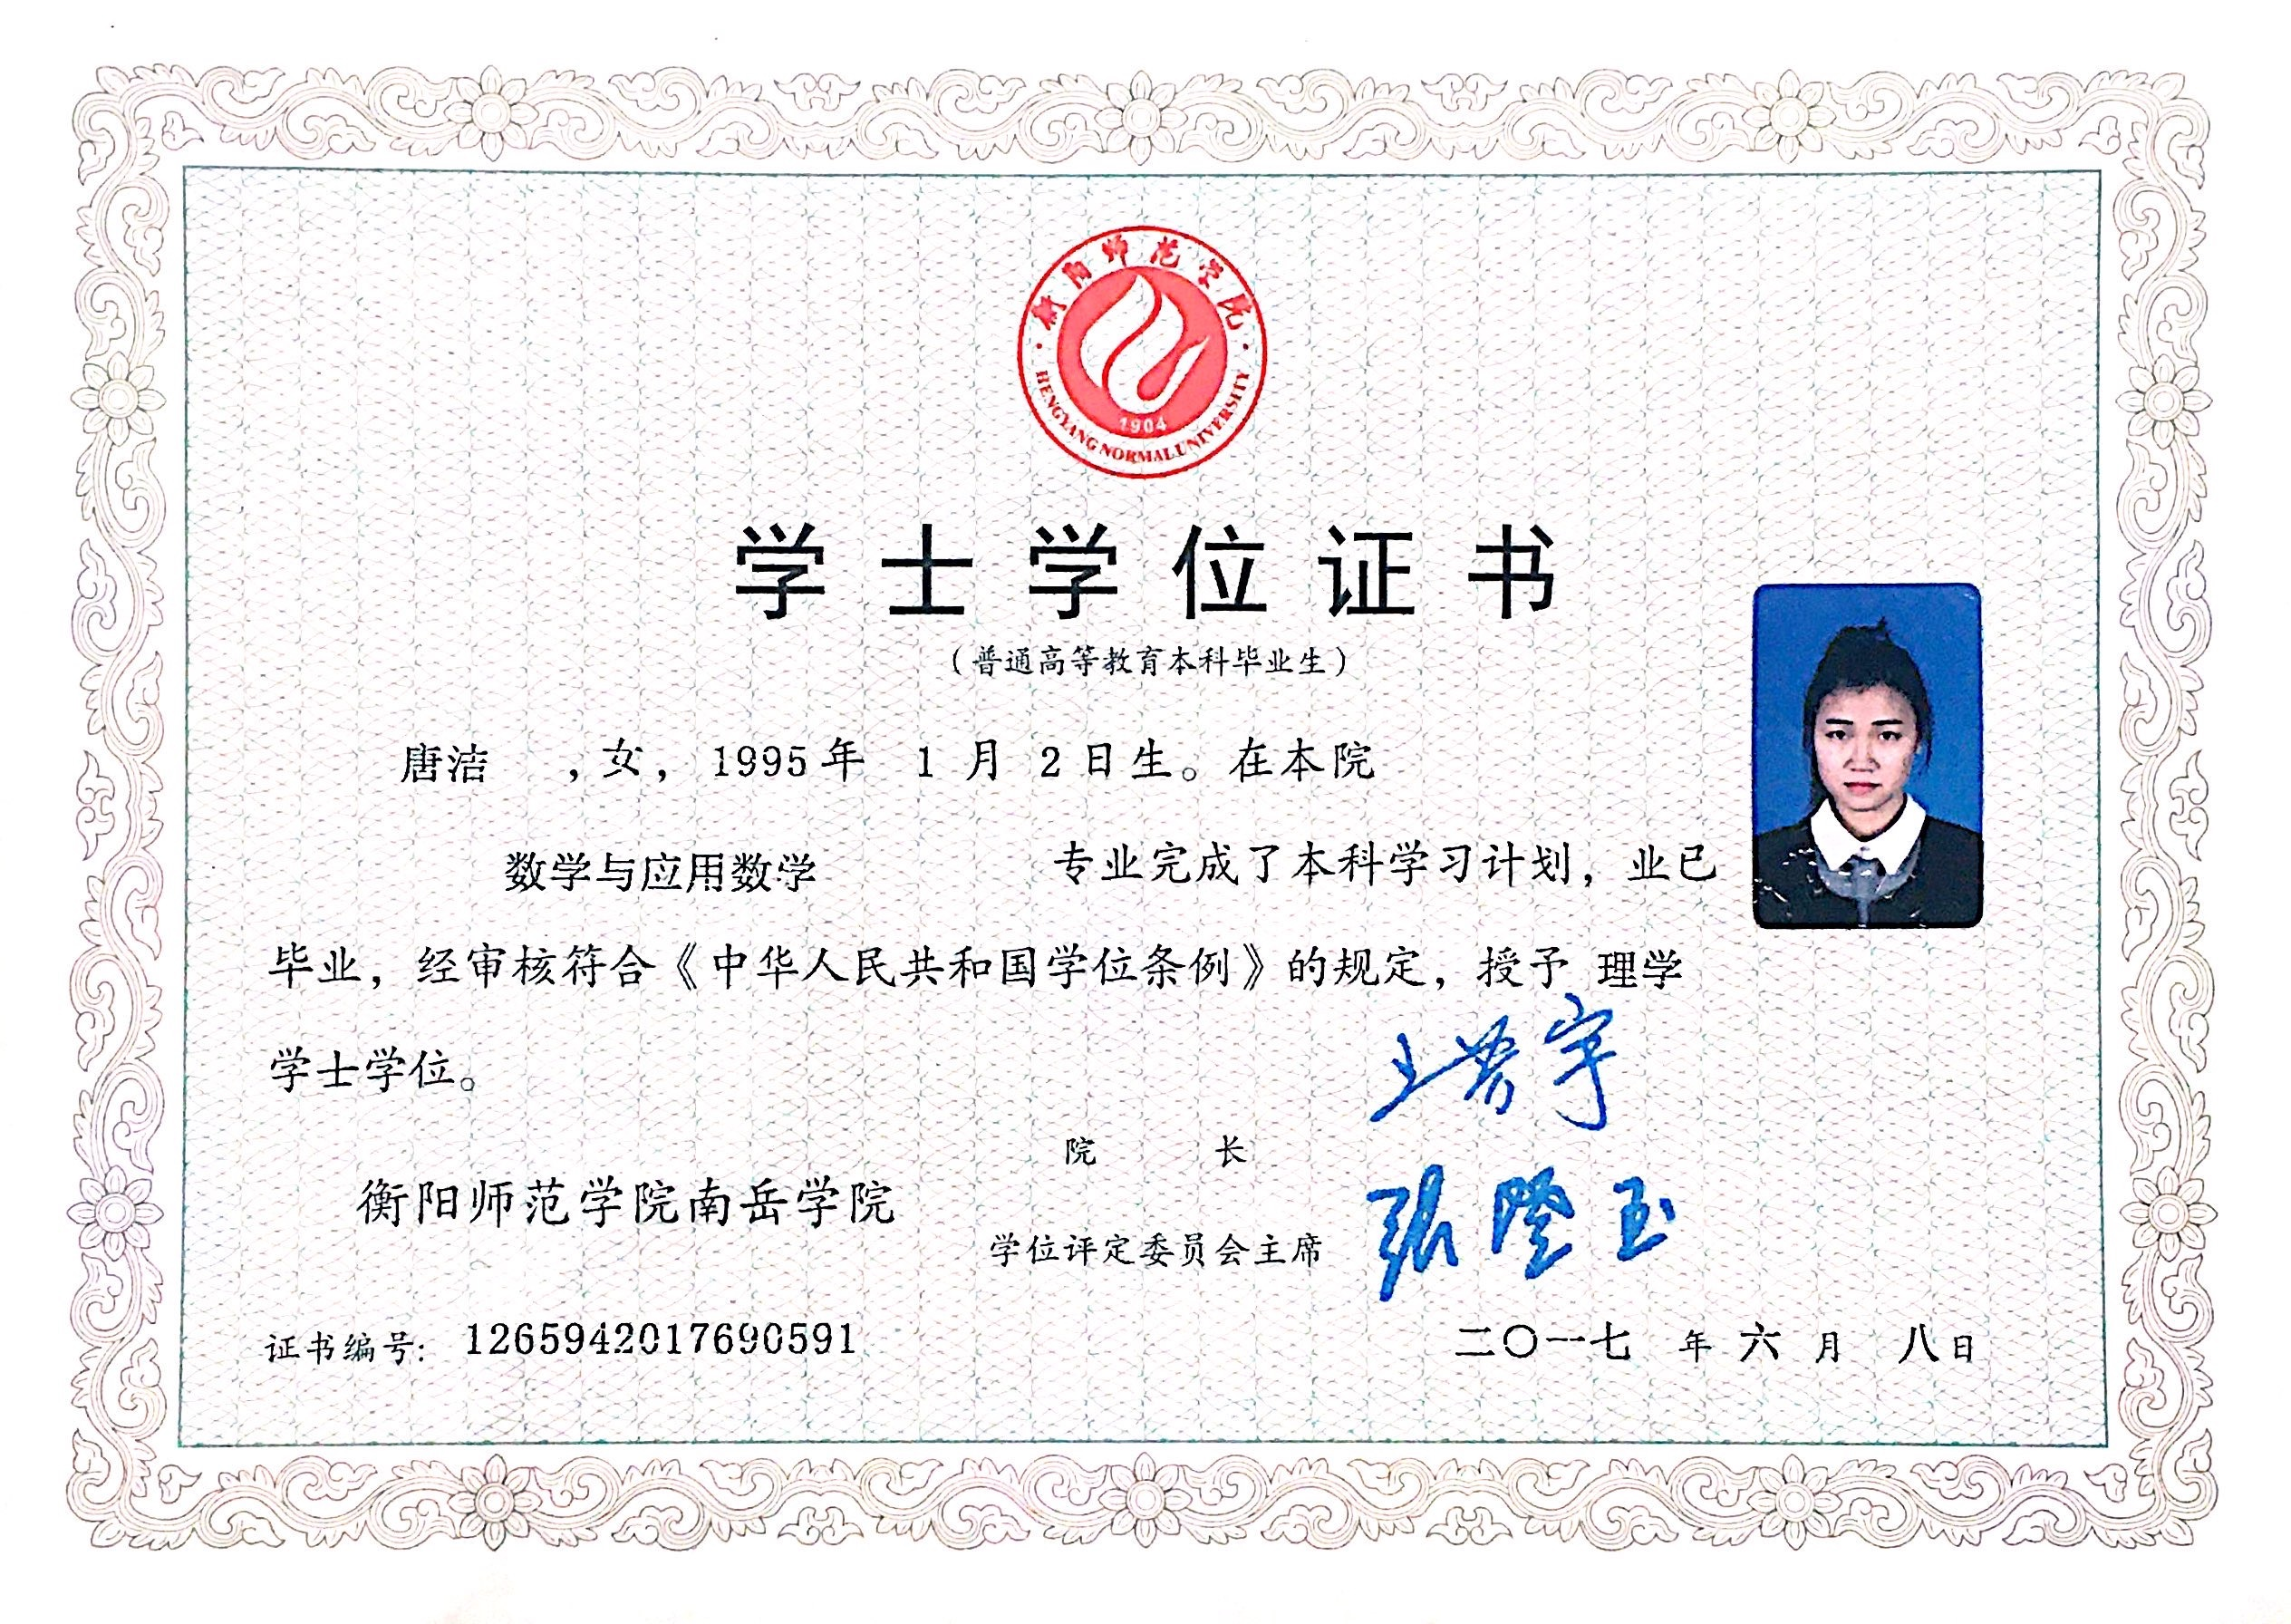
\includegraphics[scale=0.2]{figs/20170608_2.JPG }
%\end{center}


\subsection{教育部学历证书电子注册备案表}
%\begin{center}
%  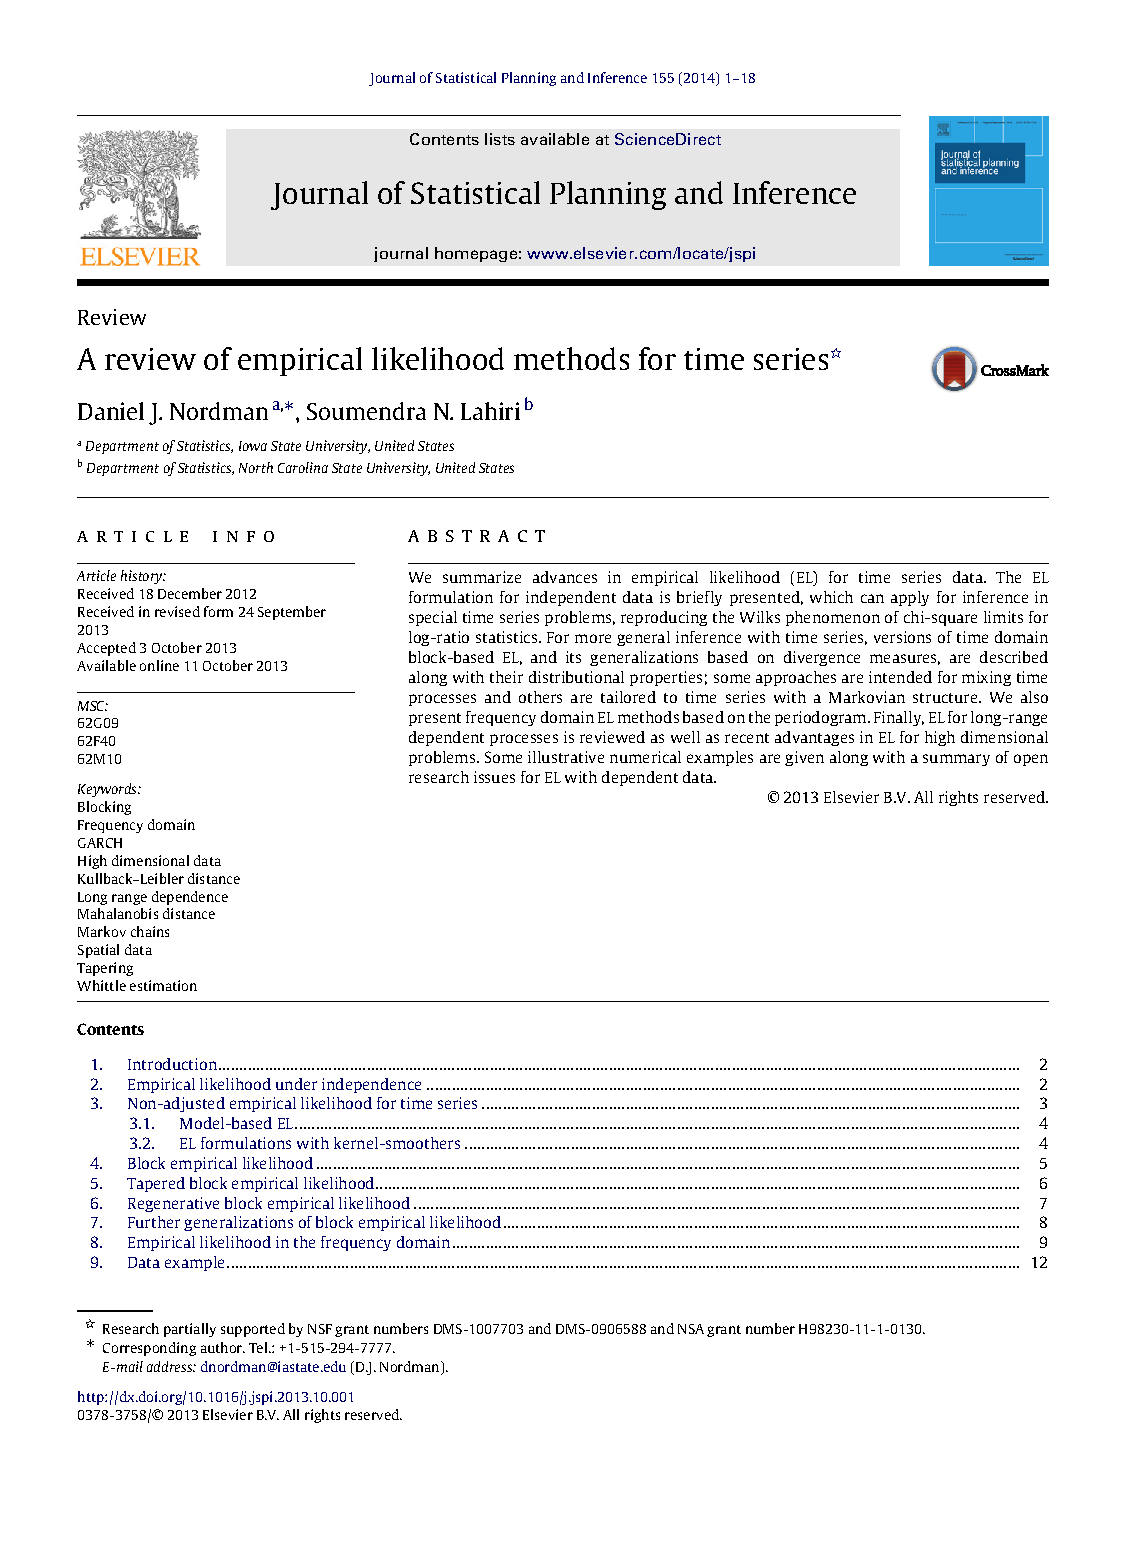
\includegraphics[scale=0.43]{figs/1.png }
%\end{center}


%\subsection{教育部学籍在线验证报告}
%\begin{center}
%  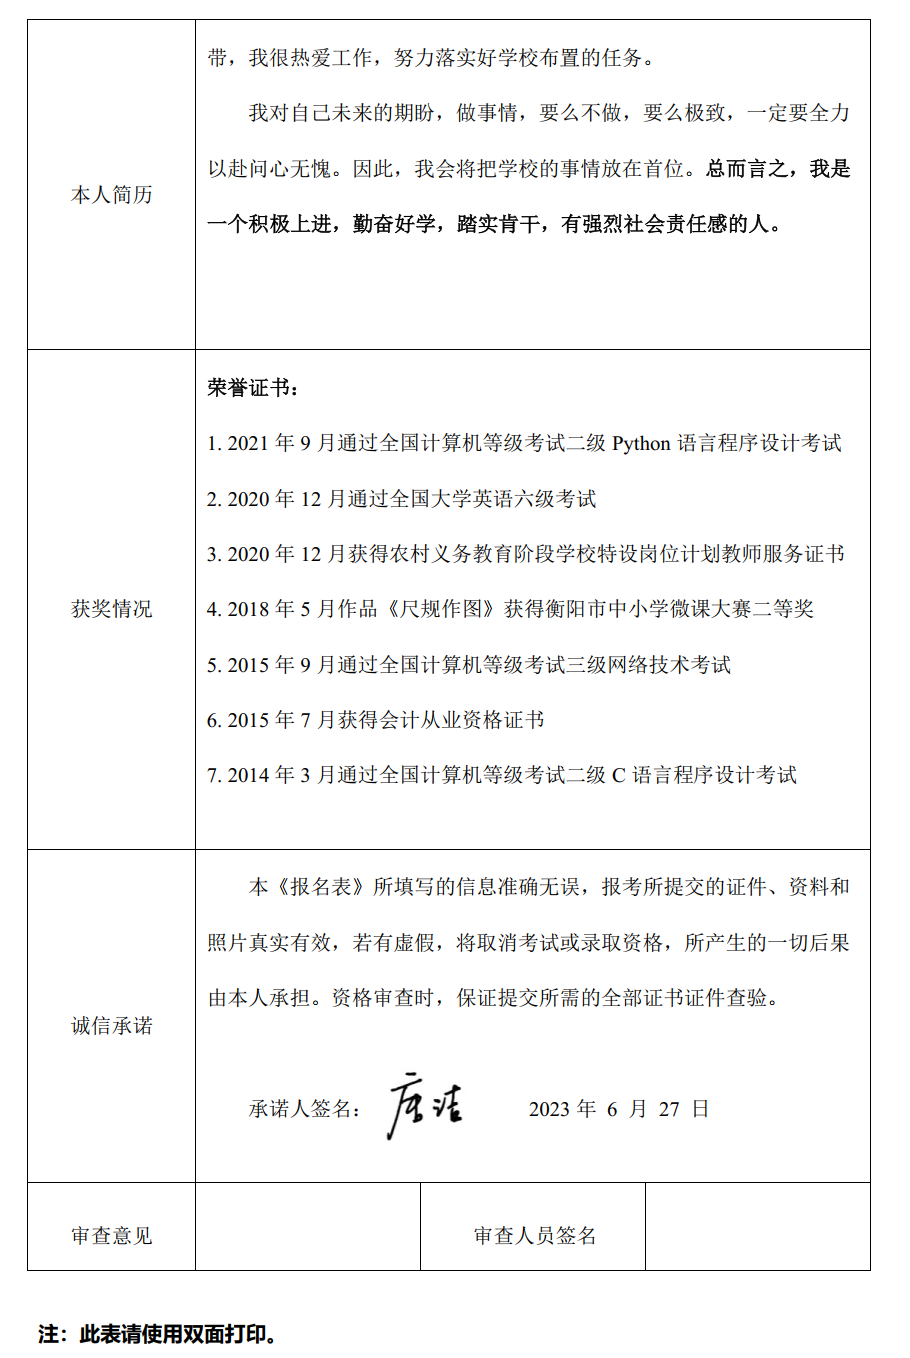
\includegraphics[scale=0.43]{figs/2.png }
%\end{center}
%
%\clearpage
%\subsection{学生证}
%\begin{center}
%  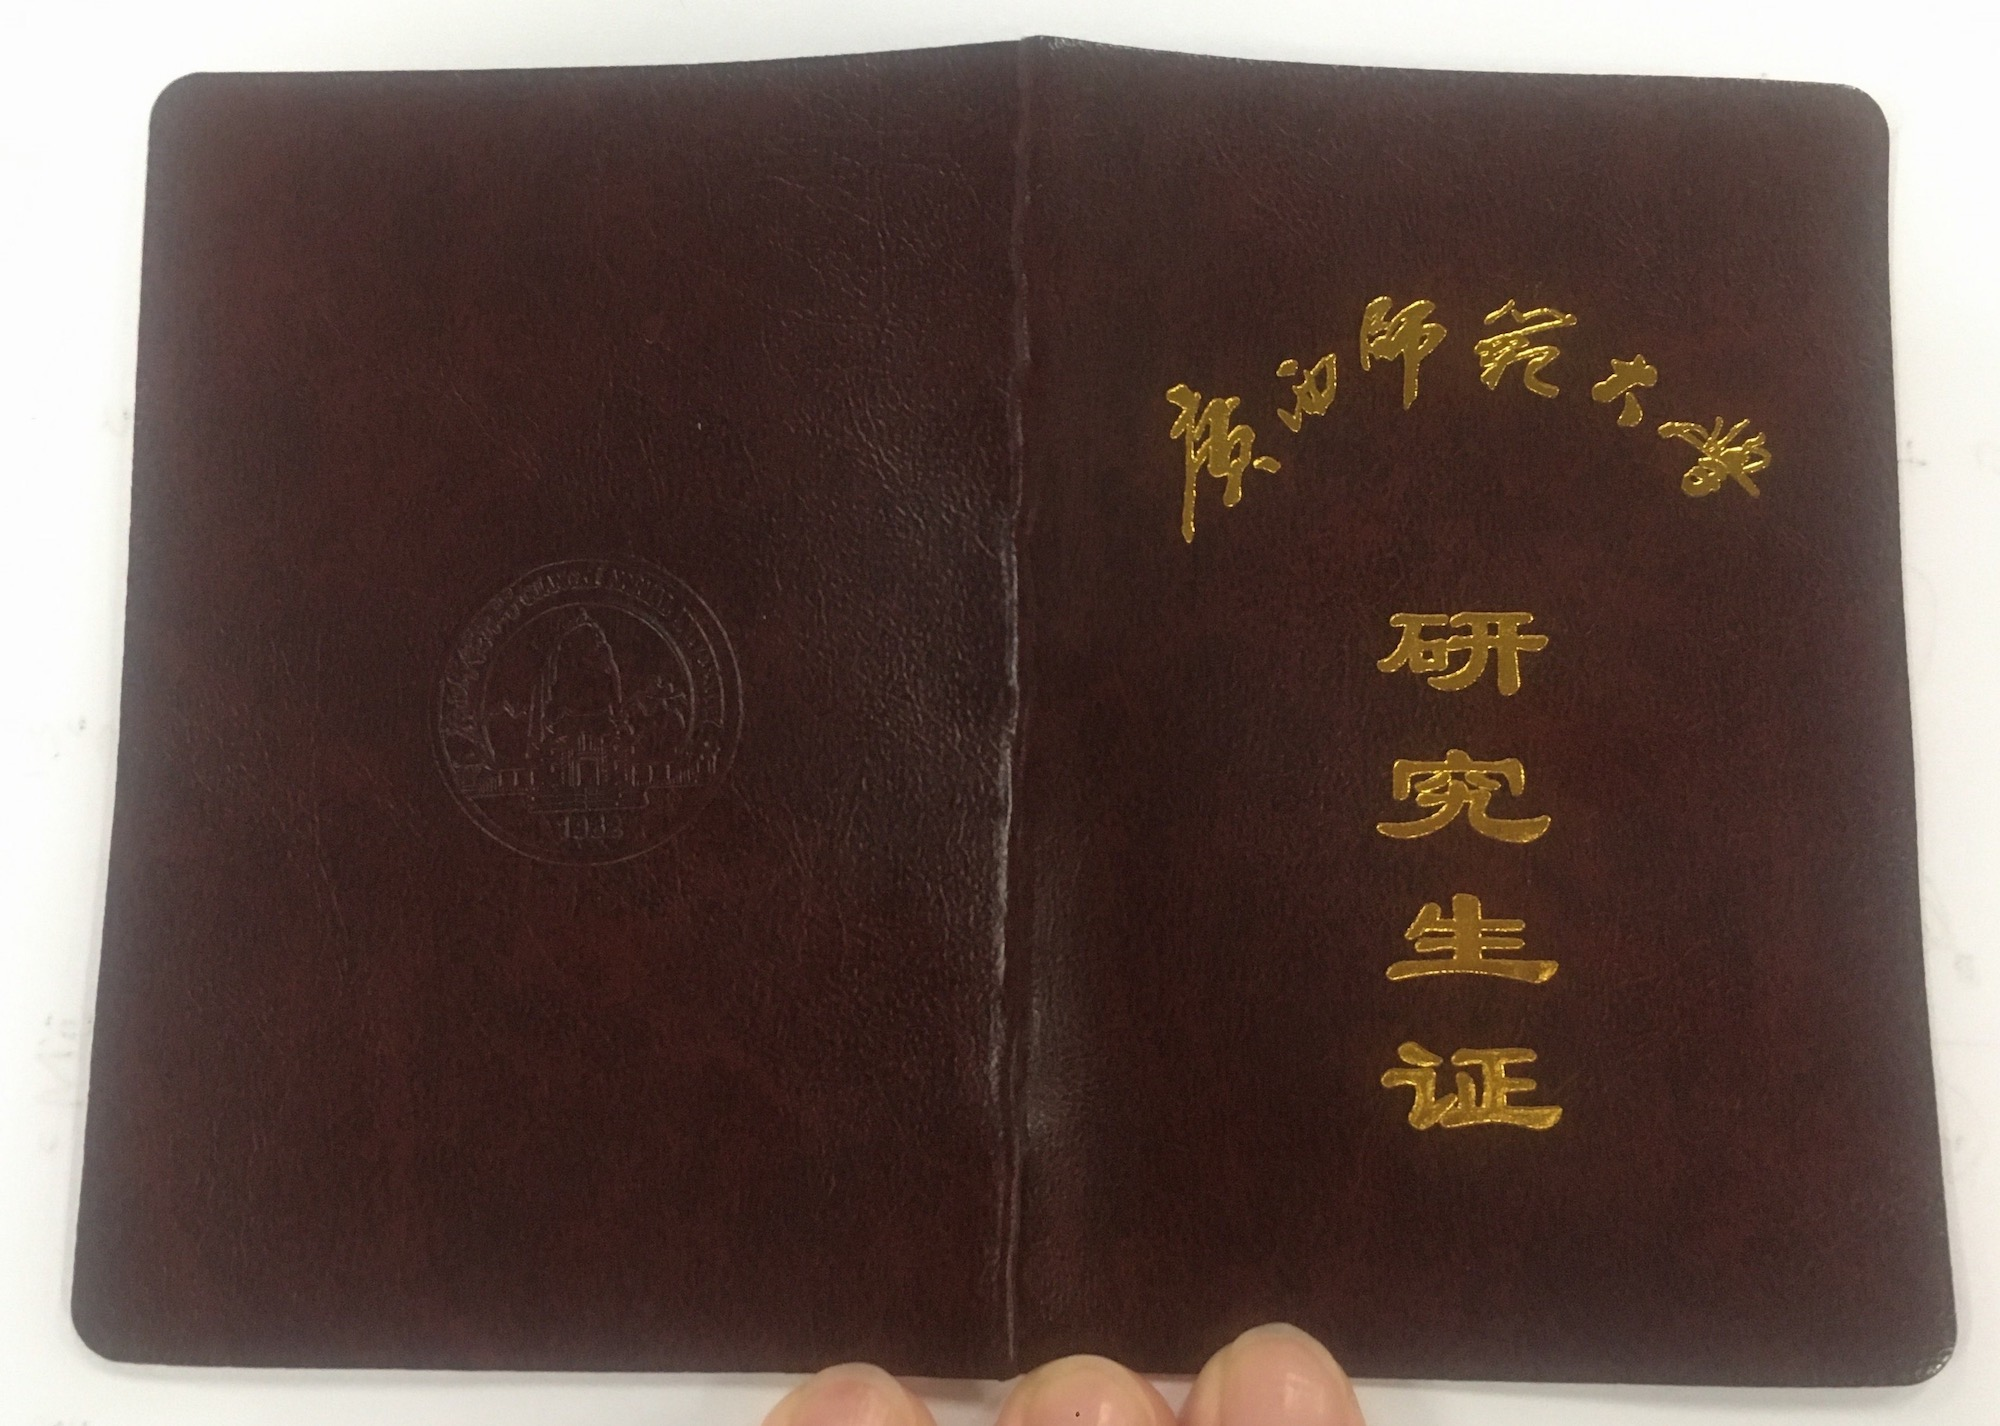
\includegraphics[scale=0.13]{figs/学生证1.JPG}
%  
%   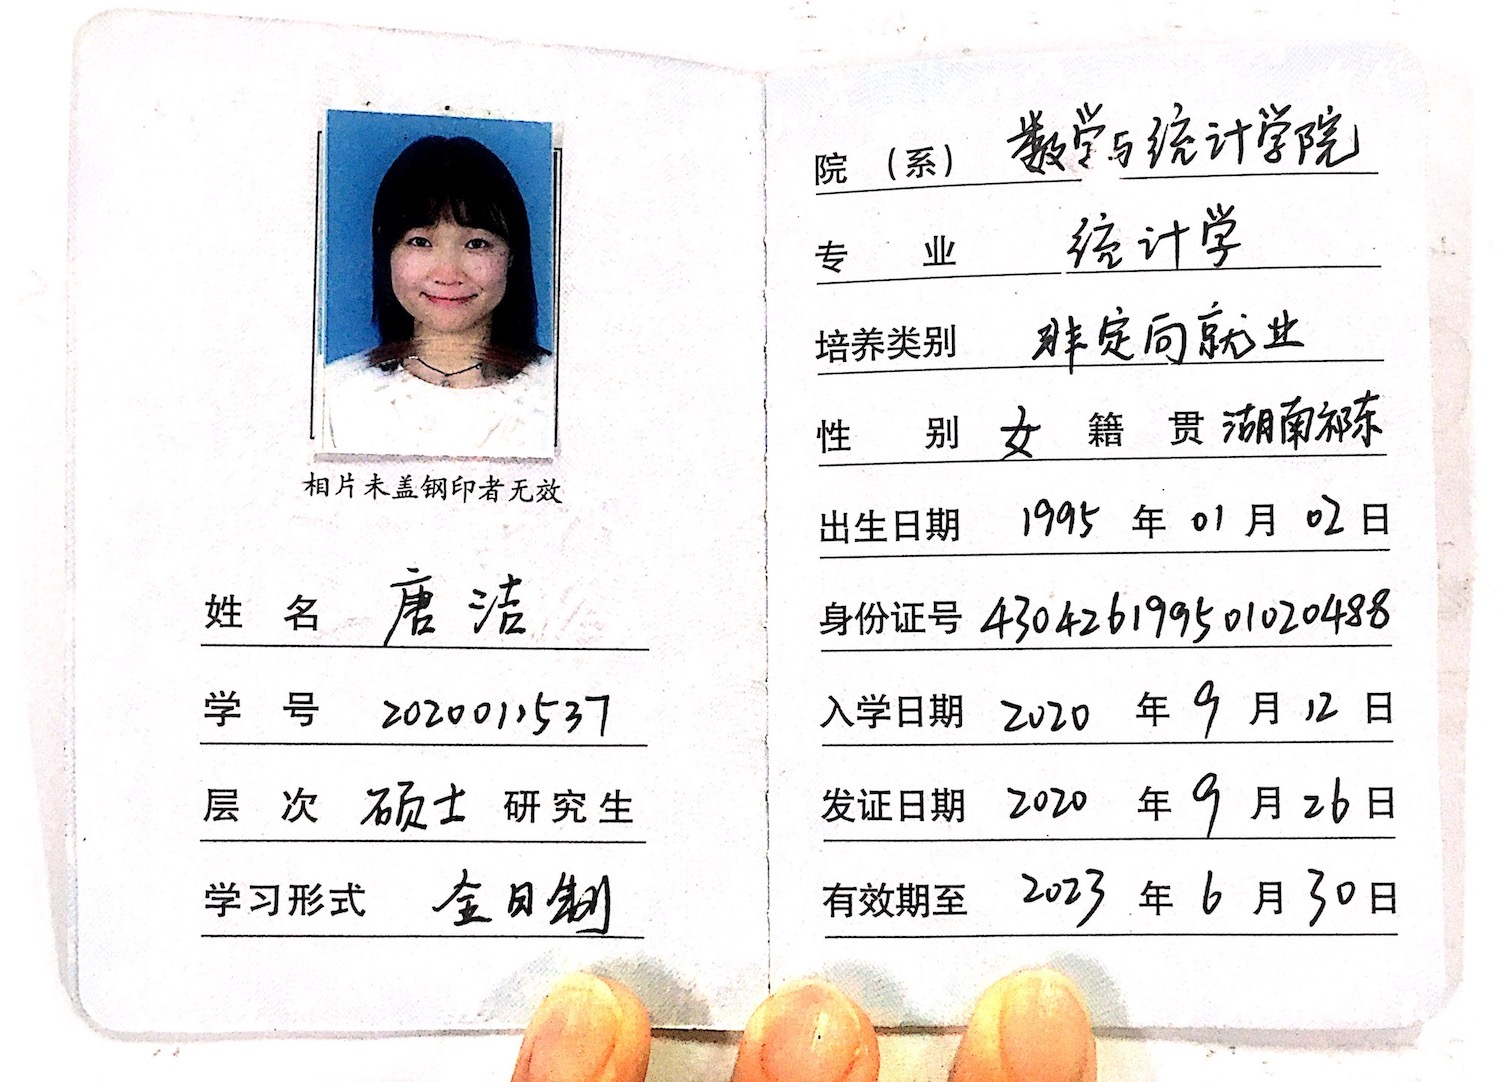
\includegraphics[scale=0.13]{figs/学生证2.JPG}
%    
%  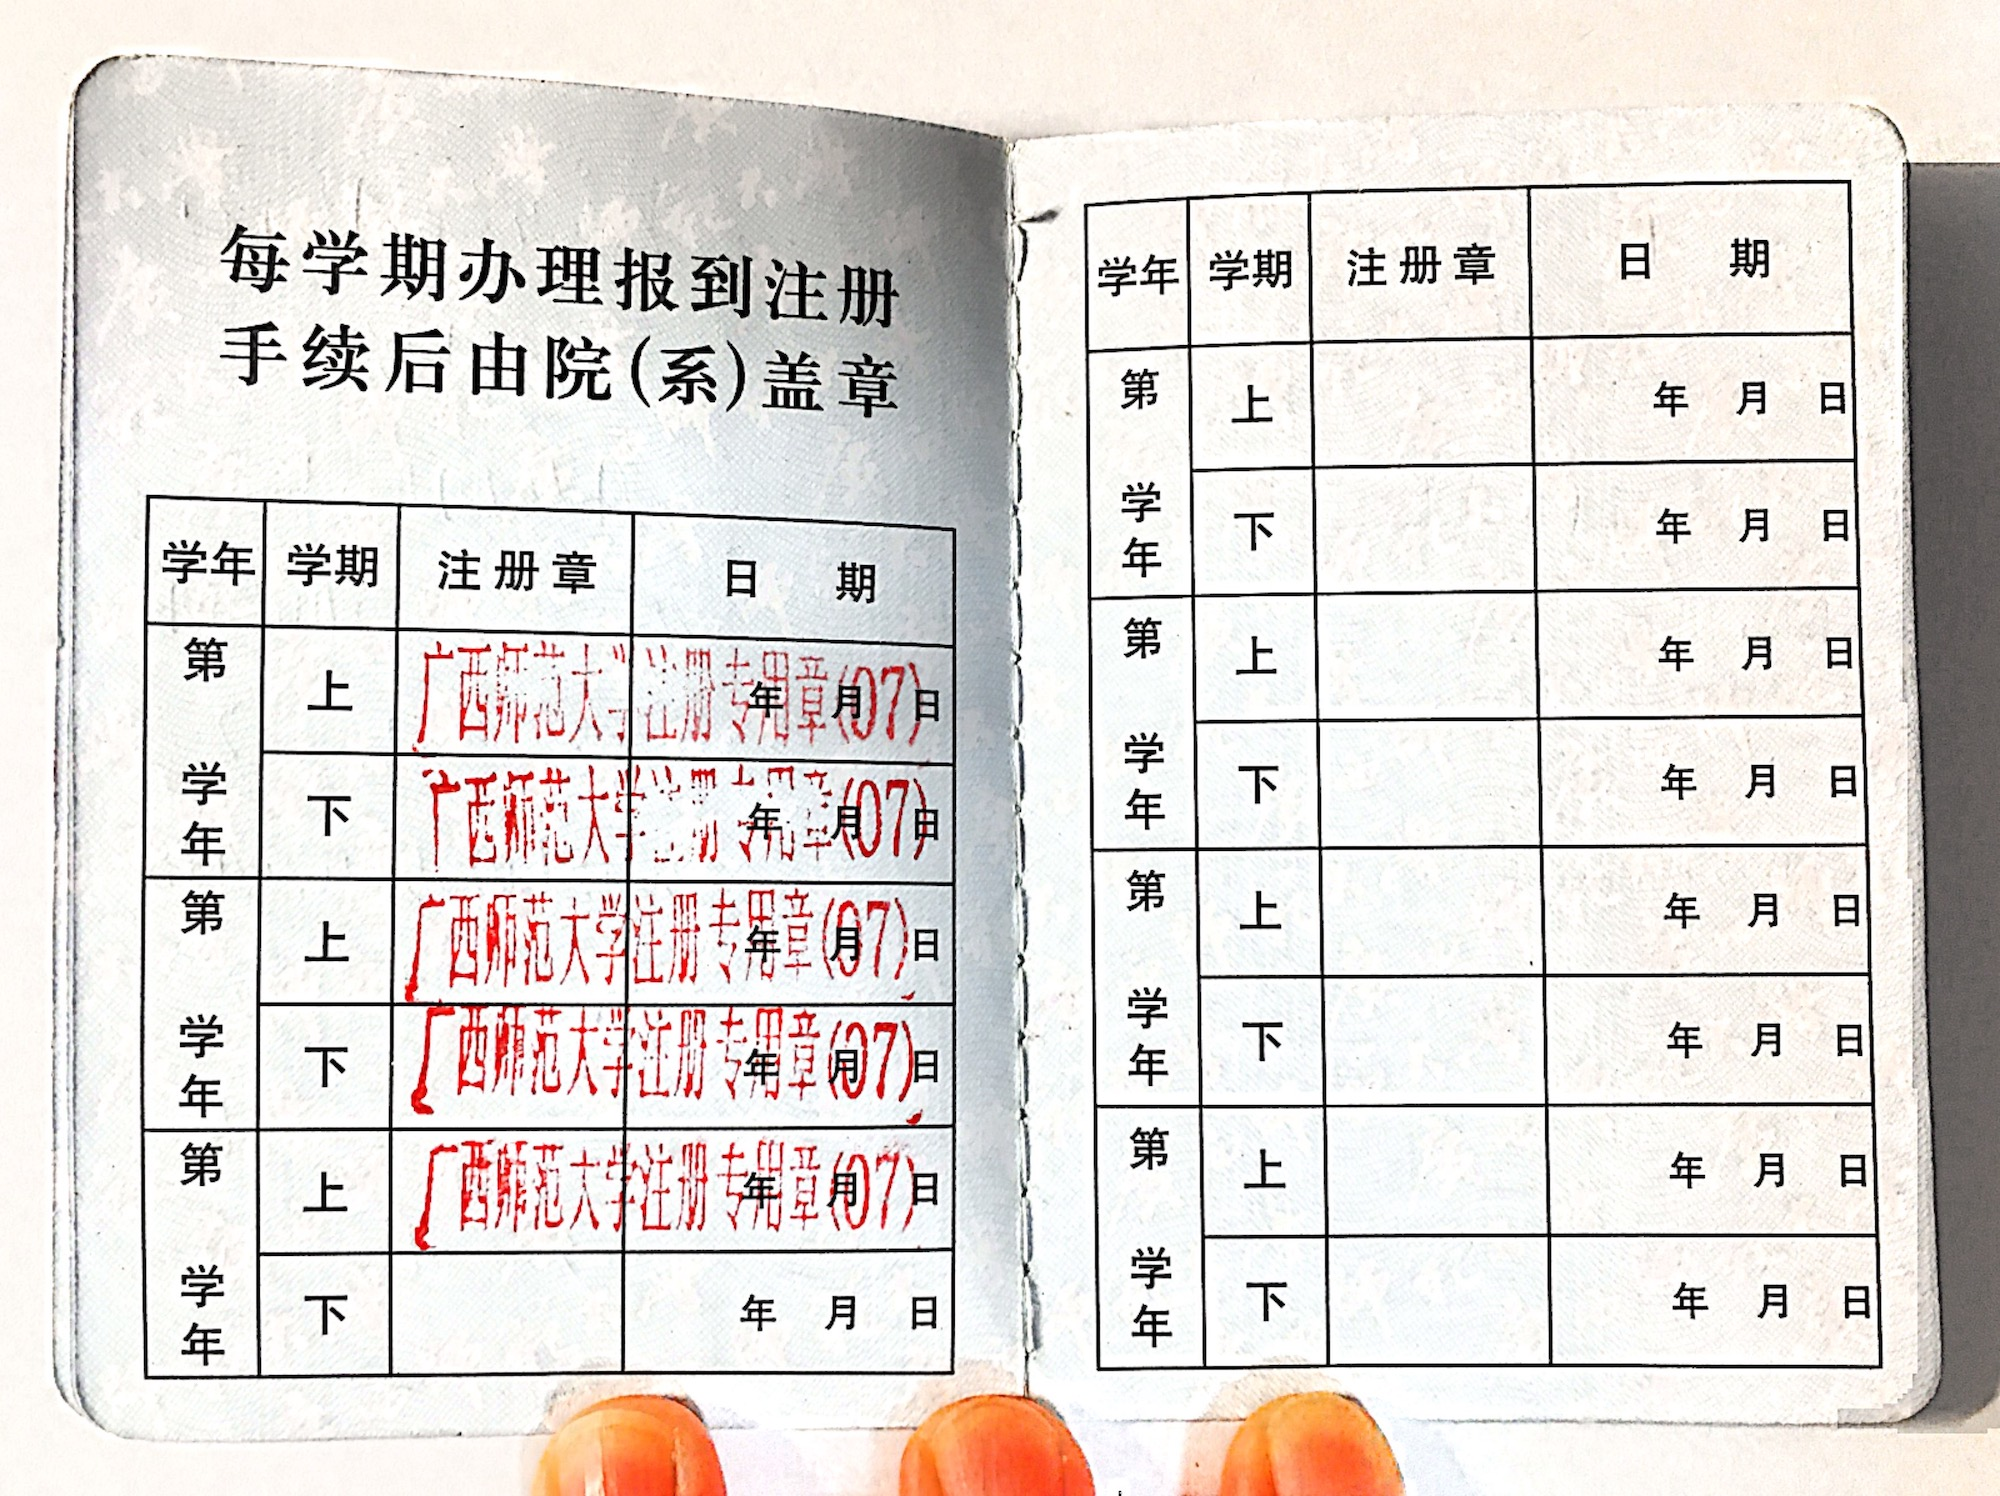
\includegraphics[scale=0.13]{figs/学生证3.JPG}
%\end{center}
%
%\clearpage
%\section{博士研究生报名登记表}
%(报考非定向的考生,单位人事部门意见无需填写)。登记表封面和封底,网上报名开始后,可在中国人民大学研招网《报考中国人民大学2023年博士生网上报名前必读》中下载,考生须在“考生签名”处亲笔签名;
%
%\clearpage
%\section{代表作原件}
%9.(可选补充材料)代表作原件1篇(含未发表的工作论文等);
%
%\clearpage
%\section{获奖证明}
% {\center \bf \kaishu      荣誉证书} 
%\be
%\item 2021年9月通过全国计算机等级考试二级Python语言程序设计考试
%
%\begin{center}
%  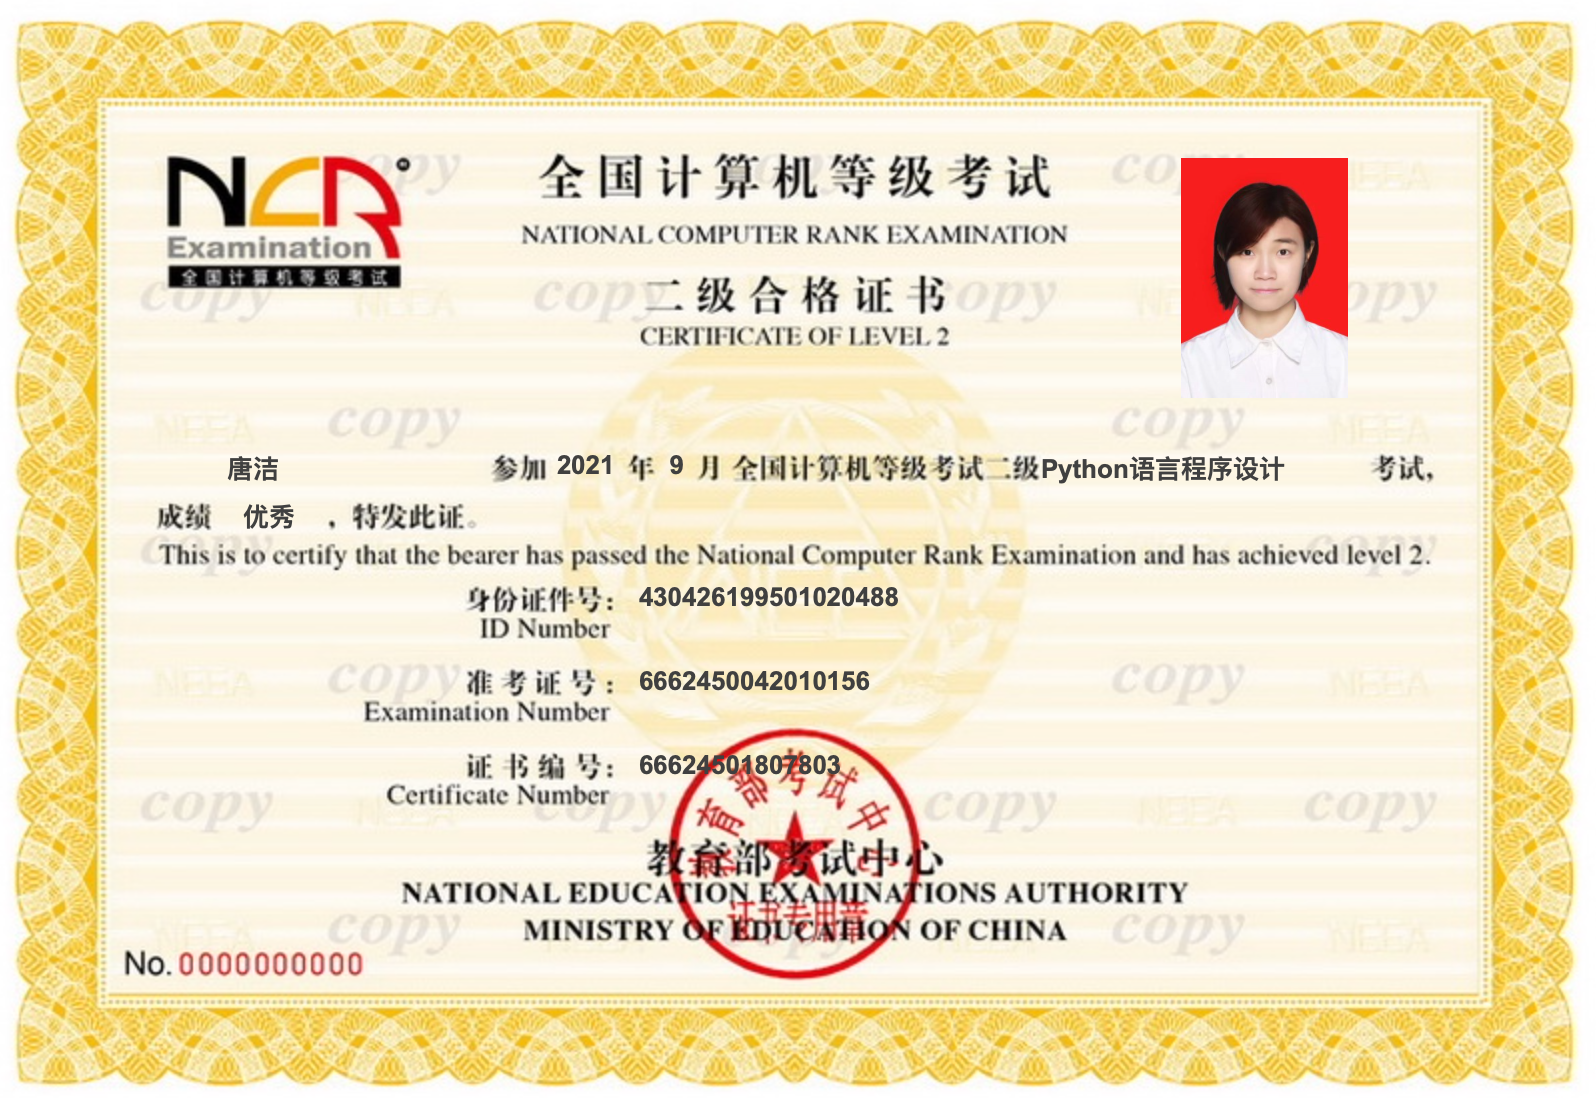
\includegraphics[scale=0.25]{figs/202109.JPG }
%\end{center}
%  
%\item 2020年12月获得农村义务教育阶段学校特设岗位计划教师服务证书
%\item 2018年5月作平《尺规作图》获得衡阳市中小学微课大赛二等奖
%\item 2017年6月具备高级中学教师资格
%\item 2015年9月通过全国计算机等级考试三级网络技术考试
%\item 2015年7月获得会计从业资格证书
%\item 2015年6⽉获得“2015年全国⼤学⽣英语竞赛”衡阳师范学院⼀等奖
%\item 2014年3⽉通过全国计算机等级考试⼆级C语⾔程序设计考试
%\ee
%
%\clearpage
%\section{承诺书}
%11.承诺书(附件1);
%\section{最后}
%12.博士生报名信息汇总表(附件2)。
%申请人须将以上1-11项申请材料按顺序合并为一个pdf文档,并以“2023年博士申请材料+姓名”命名,与第12项材料一起发送至isbd@ruc.edu.cn邮箱。材料接收截止时间为2022年12月10日17:00,逾期不予受理。

\end{document}

















































